% !TeX root = ../main.tex
% Add the above to each chapter to make compiling the PDF easier in some editors.

\chapter{Congruence Closure with Explain Operation}\label{chapter:congruence_closure}

\section{Congruence Closure Algorithm}

\section{Implementation}

For the implementation of the congruence closure algorithm, we follow the description in the paper. \cite{Nieuwenhuis}

\subsection{Modified Union Find Algorithm}

In order to implement an explain operation with a reasonable runtime for the congruence closure data structure, the paper \cite{Nieuwenhuis} introduces an alternative union-find algorithm. We will not discuss in detail the runtimes of the functions, since the main objective of this thesis is to prove the correctness of the algorithms, and for this purpose we disregarad sThe \lstinline{find} function remains the same, but for \lstinline{union} and \lstinline{explain} a new data structure is introduced, the \emph{proof forest}, i.e. a forest which has as nodes the variables, and as edges the unions that were made. The forest structure is preserved by \lstinline{union}, because redundant unions are ignored.


\subsubsection{add\_edge}
\label{subsubsection:addedge}

The proof forest has directed edges, and for each equivalence class there is a representative node, where all the edges are directed towards. To keep this invariant, each time and edge from $e$ to $e'$ is added, all the edges on the path from the root of $e$ to $e$ are reversed.
In the implementation, the proof forest is represented by a list which stores the parent of each node, exactly as in the union-find list. My implementation for adding an edge, which corresponds to the \lstinline{union} operation, is the following:

\begin{lstlisting}
function (domintros) add_edge :: "nat list ⇒ nat ⇒ nat ⇒ nat list"
  where
"add_edge pf e e' = (if pf ! e = e
                        then (pf[e := e'])
                        else add_edge (pf[e := e']) (pf ! e) e)"
  by pat_completeness auto
\end{lstlisting}

We can show that \lstinline{add_edge e e'} terminates, if the invariant \lstinline{ufa_invar} holds for the proof forest and $e$ and $e'$ do not belong to the same equivalence class.

\begin{lstlisting}
lemma add_edge_domain:
  assumes "ufa_invar l" "rep_of l e ≠ rep_of l e'"
  shows "add_edge_dom (l, e, e')"
\end{lstlisting}

\begin{proof}
It can be proven by induction on the length of the path $p$ from the root of $e$ to $e$.

In the base case there is only one node in the path, therefore $e$ must be equal to its root, therefore $pf ! e = e$, and the algorithm terminates immediately.

In the other case $e$ is not a root, then there is a path $p'$ from the root to the parent of $e$ which is shorter than the path from the root to $e$. The path $p'$ is also present in the $pf[e := e']$, because the path does not contain $e$. Also, the representative of $e$ in $pf[e := e']$ is equal to the representative of $e'$, and the representative of the parent of $e$ is still the old representative of $e$, therefore they are not in the same representative class, and we can apply the induction hypothesis and conclude that the recursive call terminates, therefore the function terminates.
\end{proof}



\tikzset{every picture/.style={line width=0.75pt}} %set default line width to 0.75pt

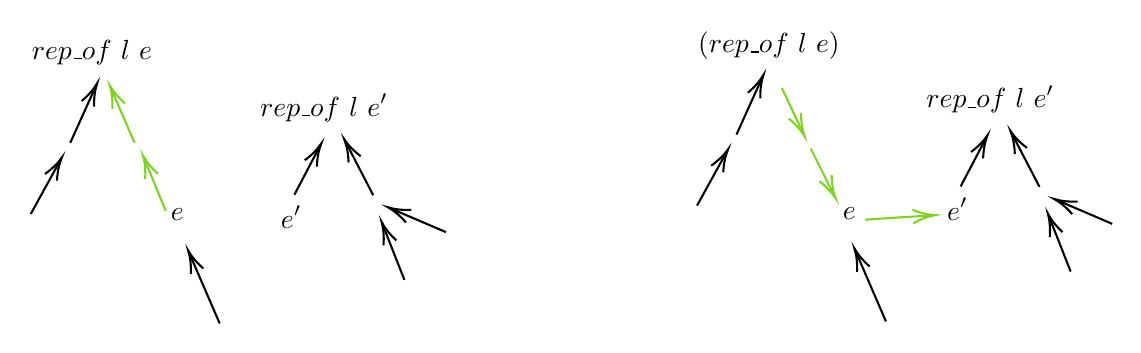
\begin{tikzpicture}[x=0.75pt,y=0.75pt,yscale=-1,xscale=1]
	%uncomment if require: \path (0,190); %set diagram left start at 0, and has height of 190

	%Straight Lines [id:da7388909588496015]
	\draw [color={rgb, 255:red, 126; green, 211; blue, 33 }  ,draw opacity=1 ]   (86,78) -- (74.79,52.07) ;
	\draw [shift={(74,50.23)}, rotate = 66.63] [color={rgb, 255:red, 126; green, 211; blue, 33 }  ,draw opacity=1 ][line width=0.75]    (10.93,-3.29) .. controls (6.95,-1.4) and (3.31,-0.3) .. (0,0) .. controls (3.31,0.3) and (6.95,1.4) .. (10.93,3.29)   ;
	%Straight Lines [id:da932845693599931]
	\draw [color={rgb, 255:red, 126; green, 211; blue, 33 }  ,draw opacity=1 ]   (101,110.77) -- (90.76,85.85) ;
	\draw [shift={(90,84)}, rotate = 67.66] [color={rgb, 255:red, 126; green, 211; blue, 33 }  ,draw opacity=1 ][line width=0.75]    (10.93,-3.29) .. controls (6.95,-1.4) and (3.31,-0.3) .. (0,0) .. controls (3.31,0.3) and (6.95,1.4) .. (10.93,3.29)   ;
	%Straight Lines [id:da8126326447235763]
	\draw    (55,78) -- (67.18,51.05) ;
	\draw [shift={(68,49.23)}, rotate = 114.32] [color={rgb, 255:red, 0; green, 0; blue, 0 }  ][line width=0.75]    (10.93,-3.29) .. controls (6.95,-1.4) and (3.31,-0.3) .. (0,0) .. controls (3.31,0.3) and (6.95,1.4) .. (10.93,3.29)   ;
	%Straight Lines [id:da6899851051736223]
	\draw    (36,112.23) -- (50.03,86.75) ;
	\draw [shift={(51,85)}, rotate = 118.85] [color={rgb, 255:red, 0; green, 0; blue, 0 }  ][line width=0.75]    (10.93,-3.29) .. controls (6.95,-1.4) and (3.31,-0.3) .. (0,0) .. controls (3.31,0.3) and (6.95,1.4) .. (10.93,3.29)   ;
	%Straight Lines [id:da19284936033329814]
	\draw    (163,103) -- (175.07,80) ;
	\draw [shift={(176,78.23)}, rotate = 117.69] [color={rgb, 255:red, 0; green, 0; blue, 0 }  ][line width=0.75]    (10.93,-3.29) .. controls (6.95,-1.4) and (3.31,-0.3) .. (0,0) .. controls (3.31,0.3) and (6.95,1.4) .. (10.93,3.29)   ;
	%Straight Lines [id:da21247734751433156]
	\draw    (201,103.23) -- (187.92,78) ;
	\draw [shift={(187,76.23)}, rotate = 62.59] [color={rgb, 255:red, 0; green, 0; blue, 0 }  ][line width=0.75]    (10.93,-3.29) .. controls (6.95,-1.4) and (3.31,-0.3) .. (0,0) .. controls (3.31,0.3) and (6.95,1.4) .. (10.93,3.29)   ;
	%Straight Lines [id:da18784825583709686]
	\draw    (216,144) -- (205.73,117.86) ;
	\draw [shift={(205,116)}, rotate = 68.55] [color={rgb, 255:red, 0; green, 0; blue, 0 }  ][line width=0.75]    (10.93,-3.29) .. controls (6.95,-1.4) and (3.31,-0.3) .. (0,0) .. controls (3.31,0.3) and (6.95,1.4) .. (10.93,3.29)   ;
	%Straight Lines [id:da43419875667135477]
	\draw    (236,121) -- (209.84,109.79) ;
	\draw [shift={(208,109)}, rotate = 23.2] [color={rgb, 255:red, 0; green, 0; blue, 0 }  ][line width=0.75]    (10.93,-3.29) .. controls (6.95,-1.4) and (3.31,-0.3) .. (0,0) .. controls (3.31,0.3) and (6.95,1.4) .. (10.93,3.29)   ;
	%Straight Lines [id:da8377415360718197]
	\draw    (127,165) -- (112.59,131.64) ;
	\draw [shift={(111.8,129.8)}, rotate = 66.64] [color={rgb, 255:red, 0; green, 0; blue, 0 }  ][line width=0.75]    (10.93,-3.29) .. controls (6.95,-1.4) and (3.31,-0.3) .. (0,0) .. controls (3.31,0.3) and (6.95,1.4) .. (10.93,3.29)   ;
	%Straight Lines [id:da9212006749144803]
	\draw [color={rgb, 255:red, 126; green, 211; blue, 33 }  ,draw opacity=1 ]   (397.86,51.57) -- (407.95,72.99) ;
	\draw [shift={(408.8,74.8)}, rotate = 244.78] [color={rgb, 255:red, 126; green, 211; blue, 33 }  ,draw opacity=1 ][line width=0.75]    (10.93,-3.29) .. controls (6.95,-1.4) and (3.31,-0.3) .. (0,0) .. controls (3.31,0.3) and (6.95,1.4) .. (10.93,3.29)   ;
	%Straight Lines [id:da9112225070236206]
	\draw [color={rgb, 255:red, 126; green, 211; blue, 33 }  ,draw opacity=1 ]   (411.8,80.8) -- (422.91,103.01) ;
	\draw [shift={(423.8,104.8)}, rotate = 243.43] [color={rgb, 255:red, 126; green, 211; blue, 33 }  ,draw opacity=1 ][line width=0.75]    (10.93,-3.29) .. controls (6.95,-1.4) and (3.31,-0.3) .. (0,0) .. controls (3.31,0.3) and (6.95,1.4) .. (10.93,3.29)   ;
	%Straight Lines [id:da026589038011743282]
	\draw    (376,74) -- (388.18,47.05) ;
	\draw [shift={(389,45.23)}, rotate = 114.32] [color={rgb, 255:red, 0; green, 0; blue, 0 }  ][line width=0.75]    (10.93,-3.29) .. controls (6.95,-1.4) and (3.31,-0.3) .. (0,0) .. controls (3.31,0.3) and (6.95,1.4) .. (10.93,3.29)   ;
	%Straight Lines [id:da4465748806717764]
	\draw    (357,108.23) -- (371.03,82.75) ;
	\draw [shift={(372,81)}, rotate = 118.85] [color={rgb, 255:red, 0; green, 0; blue, 0 }  ][line width=0.75]    (10.93,-3.29) .. controls (6.95,-1.4) and (3.31,-0.3) .. (0,0) .. controls (3.31,0.3) and (6.95,1.4) .. (10.93,3.29)   ;
	%Straight Lines [id:da8556828124311282]
	\draw    (484,99) -- (496.07,76) ;
	\draw [shift={(497,74.23)}, rotate = 117.69] [color={rgb, 255:red, 0; green, 0; blue, 0 }  ][line width=0.75]    (10.93,-3.29) .. controls (6.95,-1.4) and (3.31,-0.3) .. (0,0) .. controls (3.31,0.3) and (6.95,1.4) .. (10.93,3.29)   ;
	%Straight Lines [id:da17154675848466616]
	\draw    (522,99.23) -- (508.92,74) ;
	\draw [shift={(508,72.23)}, rotate = 62.59] [color={rgb, 255:red, 0; green, 0; blue, 0 }  ][line width=0.75]    (10.93,-3.29) .. controls (6.95,-1.4) and (3.31,-0.3) .. (0,0) .. controls (3.31,0.3) and (6.95,1.4) .. (10.93,3.29)   ;
	%Straight Lines [id:da5166223592338979]
	\draw    (537,140) -- (526.73,113.86) ;
	\draw [shift={(526,112)}, rotate = 68.55] [color={rgb, 255:red, 0; green, 0; blue, 0 }  ][line width=0.75]    (10.93,-3.29) .. controls (6.95,-1.4) and (3.31,-0.3) .. (0,0) .. controls (3.31,0.3) and (6.95,1.4) .. (10.93,3.29)   ;
	%Straight Lines [id:da8973818170227796]
	\draw    (557,117) -- (530.84,105.79) ;
	\draw [shift={(529,105)}, rotate = 23.2] [color={rgb, 255:red, 0; green, 0; blue, 0 }  ][line width=0.75]    (10.93,-3.29) .. controls (6.95,-1.4) and (3.31,-0.3) .. (0,0) .. controls (3.31,0.3) and (6.95,1.4) .. (10.93,3.29)   ;
	%Straight Lines [id:da17526153342314021]
	\draw [color={rgb, 255:red, 126; green, 211; blue, 33 }  ,draw opacity=1 ]   (438,115) -- (469.8,112.93) ;
	\draw [shift={(471.8,112.8)}, rotate = 176.28] [color={rgb, 255:red, 126; green, 211; blue, 33 }  ,draw opacity=1 ][line width=0.75]    (10.93,-3.29) .. controls (6.95,-1.4) and (3.31,-0.3) .. (0,0) .. controls (3.31,0.3) and (6.95,1.4) .. (10.93,3.29)   ;
	%Straight Lines [id:da07613740586925388]
	\draw    (448,164) -- (433.59,130.64) ;
	\draw [shift={(432.8,128.8)}, rotate = 66.64] [color={rgb, 255:red, 0; green, 0; blue, 0 }  ][line width=0.75]    (10.93,-3.29) .. controls (6.95,-1.4) and (3.31,-0.3) .. (0,0) .. controls (3.31,0.3) and (6.95,1.4) .. (10.93,3.29)   ;

	% Text Node
	\draw (35,27) node [anchor=north west][inner sep=0.75pt]   [align=left] {$\displaystyle rep\_of\ l\ e$};
	% Text Node
	\draw (102,108) node [anchor=north west][inner sep=0.75pt]   [align=left] {$\displaystyle e$};
	% Text Node
	\draw (155,107) node [anchor=north west][inner sep=0.75pt]   [align=left] {$\displaystyle e'$};
	% Text Node
	\draw (145,53) node [anchor=north west][inner sep=0.75pt]   [align=left] {$\displaystyle rep\_of\ l\ e'$};
	% Text Node
	\draw (356,23) node [anchor=north west][inner sep=0.75pt]   [align=left] {$\displaystyle (rep\_of\ l\ e)$};
	% Text Node
	\draw (425.8,107.8) node [anchor=north west][inner sep=0.75pt]   [align=left] {$\displaystyle e$};
	% Text Node
	\draw (476,103) node [anchor=north west][inner sep=0.75pt]   [align=left] {$\displaystyle e'$};
	% Text Node
	\draw (466,49) node [anchor=north west][inner sep=0.75pt]   [align=left] {$\displaystyle rep\_of\ l\ e'$};


\end{tikzpicture}


\subsubsection{add\_label}

Additionally, each edge is labeled with the input equation or the input equations which caused the adding of this edge. This is not necessary for the union-find algorithm by itself, but it will be needed by the \lstinline{explain} operation for congruence closure. There are two possible types of labels: either an equation $a = b$ was input, or two equations of the type $F(a_1, a_2) = a$ and $F(b_1, b_2) = b$, where $a_1$ and $b_1$ were already in the same equivalence class before this union, as well as $a_2$ and $b_2$. In both theses cases a union between the equivalence classes of $a$ and $b$ must be made. The labeling is implemented by using an additional list, which at each index contains the label of the outgoing edge, or \lstinline{None} if there is no outgoing edge. It is similar to the associated unions list of union-find, but it contains directly the labels instead of an index to another list.

The labels have the type \lstinline{pending_equation}, which can be either one or two equations.

\begin{lstlisting}
datatype pending_equation = One equation
  | Two equation equation
\end{lstlisting}

The name \lstinline{pending_equation} derives from the fact that it is also the type of the elements of the pending list, which will be described in the next section. Theoretically this allows also for invalid equations for example two equations of the type $a = b$ and $c = d$, but we will prove in the next sections that the equations in the labels list are always either \lstinline{One} ($a = b$) or \lstinline{Two} ($F(a_1, a_2) = a$) ($F(b_1, b_2) = b$).

Each time an edge gets added to the proof forest, the labels need to be updated as well. The function \lstinline{add_label} adds a label to the new edge, and modifies the labels for the edges which are modified by \lstinline{add_edge}:

\begin{lstlisting}
function (domintros) add_label :: "pending_equation option list ⇒ nat list ⇒ nat ⇒ pending_equation ⇒ pending_equation option list"
  where
"add_label pfl pf e lbl =
    (if pf ! e = e
        then (pfl[e := Some lbl])
        else add_label (pfl[e := Some lbl]) pf (pf ! e) (the (pfl ! e)))"
  by pat_completeness auto
\end{lstlisting}

Similarly to the \lstinline{path_to_root} function, \lstinline{add_label} has the same recursive calls as \lstinline{rep_of}, therefore it has the same domain.

\begin{lstlisting}
lemma rep_of_dom_iff_add_label_dom:
  "rep_of_dom (pf, y)  ⟷  add_label_dom (pfl, pf, y, y')"
\end{lstlisting}

\subsection{Congruence Closure Data Structure}
\label{subsection:datastructure}

For the congruence closure algorithm there are five important data structures, which are described in the following. More details on this topic can be found in \cite{Nieuwenhuis}.

\begin{itemize}
	\item \lstinline{cc_list}: the union-find list, corresponds to the \lstinline{uf_list}.

	\item \lstinline{use_list}: a two-dimensional list which contains for each representative $a$ a list of input equations $F(b_1, b_2) = b$ where the representative of $b_1$ or $b_2$ is $a$.

	\item \lstinline{lookup}: a lookup table indexed by pairs of representatives $b$ and $c$, which stores an input equation $F(a_1, a_2) = a$ such that $b$ is the representative of $a_1$ and $c$ is the representative of $a_2$, or \lstinline{None} if no such equation exists.

    \item \lstinline{pending}: equations of the type \lstinline{One} ($a = b$) or \lstinline{Two} ($F(a_1, a_2) = a$) ($F(b_1, b_2) = b$) where $a$ and $b$ need to be merged, and $a_1$ and $b_1$ are already in the same congruence class, as well as $a_2$ and $b_2$.

    \item \lstinline{proof_forest}: the proof forest as described in the previous subsection.

    \item \lstinline{pf_labels}: the labels of the proof forest as described in the previous subsection

    \item \lstinline{input}: a set of the input equation, which will be useful for some proofs in the next sections.
\end{itemize}

In the following, we shall sometimes refer to \lstinline{cc_list} as $l$, the use list as $u$, the lookup table as $t$, the pending list as $pe$, the proof forest as $pf$, the labels list for the proof forest as $pfl$ and the input as $ip$.

\subsection{Congruence Closure Algorithm}

With this data structure we can implement the merge function as described in \cite{Nieuwenhuis}.

The merge function adds the equation to pending, and then calls propagate. If the input equation is of the type $F(a_1, a_2) = a$, then there are two possibilities: if there is already an equation $F(b_1, b_2) = b$ in the lookup table at the $(rep\_of(a_1), rep\_of(a_2))$, then we know that $a_1 = b_1$ and $a_2 = b_2$, and we add $F(b_1, b_2) = b$ and $F(a_1, a_2) = a$ to pending.
On the other hand, if the respective lookup entry is \lstinline{None}, then the equation is added to the lookup table, at the index $(rep\_of(a_1), rep\_of(a_2))$ so that the next time an equation with congruent parameters is input, they will be added together to pending.

For this case distinction there is a function \lstinline{lookup_Some}, which returns \lstinline{True} if there is an entry in lookup at the index $(rep\_of(a_1), rep\_of(a_2))$ and False otherwise, and a function \lstinline{update_lookup}, which adds the equation to lookup at the index $(rep\_of(a_1), rep\_of(a_2))$.

\begin{lstlisting}
fun merge :: "congruence_closure ⇒ equation ⇒ congruence_closure"
  where
"merge ⦇cc_list = l, use_list = u, lookup = t, pending = pe, proof_forest = pf, pf_labels = pfl, input = ip⦈
(a ≈ b) =
  propagate
    ⦇cc_list = l, use_list = u, lookup = t, pending = One (a ≈ b)#pe, proof_forest = pf, pf_labels = pfl, input = insert (a ≈ b) ip⦈"

| "merge ⦇cc_list = l, use_list = u, lookup = t, pending = pe, proof_forest = pf, pf_labels = pfl, input = ip⦈
(F a$_1$ a$_2$ ≈ a) =
(if (lookup_Some t l (F a$_1$ a$_2$ ≈ a))
  then propagate ⦇cc_list = l, use_list = u, lookup = t,
            pending = link_to_lookup t l (F a$_1$ a$_2$ ≈ a)#pe, proof_forest = pf, pf_labels = pfl, input = insert (F a$_1$ a$_2$ ≈ a) ip⦈
  else ⦇cc_list = l,
          use_list = (u[rep_of l a$_1$ := (F a$_1$ a$_2$ ≈ a)#(u ! rep_of l a$_1$)])[rep_of l a$_2$ := (F a$_1$ a$_2$ ≈ a)#(u ! rep_of l a$_2$)],
          lookup = update_lookup t l (F a$_1$ a$_2$ ≈ a),
          pending = pe, proof_forest = pf, pf_labels = pfl, input = insert (F a$_1$ a$_2$ ≈ a) ip⦈
)"
\end{lstlisting}

The main part of the algorithm is executed in propagate, which recursively takes one item from pending and performs the union of the representative classes. As previously mentioned, the pending item could be either an equation of the type $a = b$, or two equations of the type $F(a_1, a_2) = a$ and $F(b_1, b_2) = b$, where $a_1$ and $a_2$ are already in the same representative class as $b_1$ and $b_2$ respectively. In both cases the representative classes of $a$ and $b$ need to be merged. The functions \lstinline{left} and \lstinline{right} simply retrieve $a$ and $b$ from either of the two types of pending equations. If $a$ and $b$ are already in the same representative class, nothing needs to be done, otherwise the union is performed. For more clarity, I defined the union separately as \lstinline{propagate_step}.

\begin{lstlisting}
function propagate :: "congruence_closure ⇒ congruence_closure"
  where
"propagate ⦇cc_list = l, use_list = u, lookup = t, pending = [], proof_forest = pf, pf_labels = pfl, input = ip⦈ =
⦇cc_list = l, use_list = u, lookup = t, pending = [], proof_forest = pf, pf_labels = pfl, input = ip⦈"
| "propagate
⦇cc_list = l, use_list = u, lookup = t, pending = (eq # pe), proof_forest = pf, pf_labels = pfl, input = ip⦈ =
(let a = left eq; b = right eq in
  (if rep_of l a = rep_of l b
    then propagate ⦇cc_list = l, use_list = u, lookup = t, pending = pe, proof_forest = pf, pf_labels = pfl, input = ip⦈
    else
      propagate (propagate_step l u t pe pf pfl ip a b eq)
))"
  by pat_completeness auto
\end{lstlisting}

Concerning the union, we disregard some optimisations, namely the path compression and the optimisation which considers the size of the representative classes in order to choose in which direction to add the union edge. These optimisations are not relevant for the correctness of the algorithm, and they could later be added to a refinement of the algorithm.

The union consists of the previously discussed \lstinline{ufa_union}, \lstinline{add_edge} and \lstinline{add_label}, as well as a loop which moves all elements from the use list of the representative of $a$ to either the representative of $b$, or to pending. This is necessary, because the old representative of $a$ is not a representative any more, and its new representative is  $rep\_of(l, b)$.

\begin{lstlisting}
abbreviation propagate_step
  where
"propagate_step l u t pe pf pfl ip a b eq ≡
  propagate_loop (rep_of l b) (u ! rep_of l a)
    ⦇cc_list = ufa_union l a b,
    use_list = u[rep_of l a := []],
    lookup = t,
    pending = pe,
    proof_forest = add_edge pf a b,
    pf_labels = add_label pfl pf a eq,
    input = ip⦈"
\end{lstlisting}

The loop is defined as a recursive function, which considers each element of the use list of $rep\_of(l, a)$, and either adds it to the use list and the lookup table, or if there is already an entry in lookup, then that entry together with the current equation are added to pending.

\begin{lstlisting}
fun propagate_loop
  where
"propagate_loop rep_b (u1 # urest)
⦇cc_list = l, use_list = u, lookup = t, pending = pe, proof_forest = pf, pf_labels = pfl, input = ip⦈
=
  propagate_loop rep_b urest (
    if (lookup_Some t l u1)
    then
      ⦇cc_list = l, use_list = u, lookup = t,
            pending = link_to_lookup t l u1#pe,
            proof_forest = pf, pf_labels = pfl, input = ip⦈
    else
      ⦇cc_list = l,
            use_list = u[rep_b := u1 # (u ! rep_b)],
            lookup = update_lookup t l u1,
            pending = pe, proof_forest = pf, pf_labels = pfl, input = ip⦈
)"
| "propagate_loop _ [] cc = cc"
\end{lstlisting}

The function \lstinline{are_congruent} returns \lstinline{True} if an equation is in the congruence closure of all the input equations so far. It simply checks if the elements have the same representative or if they have the same representative as the correspondent entry in lookup.

\begin{lstlisting}
fun are_congruent :: "congruence_closure ⇒ equation ⇒ bool"
  where
"are_congruent ⦇cc_list = l, use_list = u, lookup = t, pending = pe, proof_forest = pf, pf_labels = pfl, input = ip⦈ (a ≈ b) =
    (rep_of l a = rep_of l b)"
| "are_congruent ⦇cc_list = l, use_list = u, lookup = t, pending = pe, proof_forest = pf, pf_labels = pfl, input = ip⦈ (F a$_1$ a$_2$ ≈ a) =
    (case lookup_entry t l a$_1$ a$_2$ of
      Some (F b$_1$ b$_2$ ≈ b) ⇒ (rep_of l a = rep_of l b)
    | None ⇒ False
)"
\end{lstlisting}

\section{Correctness Proof}

\subsection{Invariants}

At this point we can already prove some properties of the congruence closure data structure. Our approach this time is different than the one for the union-find algorithm. Instead of defining an induction rule like in the union find section and then prove the properties through the induction rule, we define the properties as invariants and then prove that they remain invariant after applying merge. For each invariant, we need to follow the same steps:

\begin{enumerate}
	\item Prove that the invariant holds for the initial empty congruence closure.

	\item Prove that if the invariant holds before the merge operation, it also holds after the merge operation. Below is a list of what needs to be proven:
    \begin{enumerate}
        \item The invariant holds after one step in the \lstinline{propagate_loop}. We shall refer to the two possible cases as \lstinline{loop1} and \lstinline{loop2}.
    	\item The invariant holds after the entire \lstinline{propagate_loop}.
    	\item The invariant holds for the parameters of \lstinline{propagate_loop} in \lstinline{propagate_step}. We shall refer to the this case as \lstinline{mini_step}.
    	\item It holds after \lstinline{propagate_step}.
    	\item It holds after \lstinline{propagate}.
    	\item And finally, it holds after \lstinline{merge}.
    \end{enumerate}
\end{enumerate}

After having defined all the invariants and proven the above properties, we can put all the invariants together in the invariant \lstinline{cc_invar} and prove the following two theorems, which state exactly the two properties described above for the invariant \lstinline{cc_invar}:

\begin{lstlisting}
theorem cc_invar_initial_cc: "cc_invar (initial_cc n)"
\end{lstlisting}

\begin{lstlisting}
theorem cc_invar_merge:
  assumes "cc_invar cc" "valid_vars eq (nr_vars cc)"
  shows "cc_invar (merge cc eq)"
\end{lstlisting}

Let us now look at the concrete invariants. Each list in the data structure has an invariant which states that all the elements which are in the list are in bounds. This is easy to prove if we assume that all the input equations contain only valid elements.

One of the invariants is the usual \lstinline{ufa_invar} that we know from the union-find algorithm. The \lstinline{ufa_invar} holds for the \lstinline{cc_list} and the \lstinline{proof_forest}. These two are only modified before entering the in the \lstinline{mini_step}, and we already proved previously that the \lstinline{ufa_invar} holds after \lstinline{ufa_union} (section union find from AFP TODO) and after \lstinline{add_edge} (Subsection \ref{subsubsection:addedge}). Therefore it also holds after \lstinline{merge}.

We define a new invariant \lstinline{inv_same_rep_classes}, which states, as the name suggests, that the union-find forest and the proof forest represent the same equivalence classes:

\begin{lstlisting}
rep_of l i = rep_of l j ⟷ rep_of pf i = rep_of pf j
\end{lstlisting}

In order to prove this, given that the two lists are only modified during the \lstinline{mini_step}, it is sufficient to show that \lstinline{ufa_union l x y} and \lstinline{add_edge pf x y} have the same behaviour. The theory \lstinline{Union_Find} from the AFP\cite{Sep} already provides the following lemma for \lstinline{ufa_union}:

\begin{lstlisting}
lemma ufa_union_aux:
  "rep_of (ufa_union l x y) i =
    (if rep_of l i = rep_of l x then rep_of l y else rep_of l i)"
\end{lstlisting}

We can show a similar lemma for \lstinline{add_edge}:

\begin{lstlisting}
lemma rep_of_add_edge_aux:
   assumes "rep_of l x ≠ rep_of l y"
   shows "rep_of (add_edge l x y) i =
     (if rep_of l i = rep_of l x then rep_of l y else rep_of l i)"
\end{lstlisting}

The additional assumption \lstinline{"rep_of l x ≠ rep_of l y"} does not cause problems, because \lstinline{add_edge} is only used within \lstinline{propagate_step}, and \lstinline{propagate_step} is only executed if \lstinline{"rep_of l x ≠ rep_of l y"}.

\begin{proof}
We already showed that the function terminates in Subsection \ref{subsubsection:addedge}, therefore we can prove it by induction on \lstinline{add_edge}.

TODO describe the proof.
\end{proof}

Additionally, for each data structure there is an invariant which states the properties which were informally described in Subsection \ref{subsection:datastructure}.

For the use list, the invariant states that for each representative $a$, its use list only contains equations of the type $F(b_1, b_2) = b$, where $a$ is the representative of either $b_1$ or $b_2$.

\begin{proof}
In order to prove the use list invariant, we can follow the steps described earlier. For the correctness proof after the \lstinline{propagate_loop}, I needed to add an additional assumption that the second parameter only contains equations of the type $F(a_1, a_2) = a$ and the representative of either $a_1$ or $a_2$ is $rep\_of(l, b)$ (where $b$ is the right side of the equation which is being propagated). This follows from the facts that the parameter of \lstinline{propagate_loop} was $(u ! rep\_of(l, a))$, and the new representative of $a$ after the union is $b$.

With this assumption I could show that each time an equation gets added to the use list in the \lstinline{propagate_loop}, it is a valid equation.

In the proof after the merge operation, the use list is only modified in the third case, and only equations of a valid form are added to $rep\_of(l, a_1)$  and r$rep\_of(l, a_2)$. Therefore all the necessary properties hold for these new equations.

For the remaining cases, use list is either unchanged, or something is removed from it, therefore the invariant trivially holds.
\end{proof}

The invariant for lookup is similar, it states that each entry in the lookup table at index $(i, j)$, for representatives $i$ and $j$, is either \lstinline{None} or is an equation of the form $F(a_1, a_2) = a$ where the representative of $a_1$ is $i$ and the representative of $a_2$  is $j$.

\begin{proof}
Each time an equation is added to lookup, it has the desired form and it is added to the index $(rep\_of(l, a_1), rep\_of(l, a_2))$. This happens in the \lstinline{propagate_loop} and in \lstinline{merge}. In the \lstinline{propagate_loop}, the added equation derives from the use list, for which we proved with the previous invariant that its equations have the desired form. In merge, only the equations of the type $F(a_1, a_2) = a$ are added to lookup.
\end{proof}

For pending, the invariant states that the equations are either of the form \lstinline{One} ($a = b$) or \lstinline{Two} ($F(a_1, a_2) = a$) ($F(b_1, b_2) = b$) where $rep\_of(l, a_1) = rep\_of(l, b_1)$ and $rep\_of(l, a_2) = rep\_of(l, b_2)$: It is important to know that they are in the same representative class, because TODO

\begin{proof}
We need to show that in the \lstinline{propagate_loop} the equation $u1$ we add to pending has a valid format. We know that $u1$ derives from the use list, therefore it is of the form $F(a_1, a_2) = a$. Then we link to it the lookup entry at the index $(rep\_of(l, a_1), rep\_of(l, a_2))$. From the lookup invariant we know that there is an entry of the form $F(b_1, b_2) = b$ at this index where $rep\_of(l, a_1) = rep\_of(l, b_1)$ and $rep\_of(l, a_2) = rep\_of(l, b_2)$. This shows that they are valid equations for pending.

The same holds for the equations added to pending in merge.
\end{proof}

There is also an invariant which states that the \lstinline{cc_list}, the first dimension of the use list, both dimensions of lookup, the proof forest and the \lstinline{pf_labels} have the same length. This was trivial to prove, given that the algorithm never changes the length of the lists, and initially the lists have the same length.

All the above-mentioned invariants hold trivially for the initial case, given that all the data structures are empty or contain only \lstinline{None} in the beginning.

The remaining invariants will be described later on, when they become relevant.


\subsection{Abstract Formalisation of Congruence Closure}
\label{subsection:abstraction}

In order to prove the correctness of the algorithm, we define an abstraction of congruence closure. We cannot use any previouly defined definitions, because the data structure that we use can only represent a subset of all possible equations, for example it cannot represent equations of the type $a = F(b, c)$ or $F (F (a, b), c) = d$. For this reason, we define an inductive set which represents the congruence closure of a set of equations and only uses the our restricted definition of equation.

\begin{lstlisting}
inductive_set Congruence_Closure :: "equation set ⇒ equation set" for S
  where
    base: "eqt ∈ S ⟹ eqt ∈ Congruence_Closure S"
  | reflexive: "(a ≈ a) ∈ Congruence_Closure S"
  | symmetric: "(a ≈ b) ∈ Congruence_Closure S ⟹ (b ≈ a) ∈ Congruence_Closure S"
  | transitive1: "(a ≈ b) ∈ Congruence_Closure S ⟹ (b ≈ c) ∈ Congruence_Closure S
⟹ (a ≈ c) ∈ Congruence_Closure S"
  | transitive2: "(F a$_1$ a$_2$ ≈ b) ∈ Congruence_Closure S ⟹ (b ≈ c) ∈ Congruence_Closure S
⟹ (F a$_1$ a$_2$ ≈ c) ∈ Congruence_Closure S"
  | transitive3: "(F a$_1$ a$_2$ ≈ a) ∈ Congruence_Closure S
⟹ (a$_1$ ≈ b$_1$) ∈ Congruence_Closure S ⟹ (a$_2$ ≈ b$_2$) ∈ Congruence_Closure S
⟹ (F b$_1$ b$_2$ ≈ a) ∈ Congruence_Closure S"
  | monotonic: "(F a$_1$ a$_2$ ≈ a) ∈ Congruence_Closure S ⟹ (F a$_1$ a$_2$ ≈ b) ∈ Congruence_Closure S
⟹ (a ≈ b) ∈ Congruence_Closure S"
\end{lstlisting}

The following proof rule follows directly from the definition of Congruence Closure, and proved to be very useful for multiple proofs:

\begin{lstlisting}
lemma Congruence_Closure_eq[case_names left right]:
  assumes "⋀ a. a ∈ A ⟹ a ∈ Congruence_Closure B"
    "⋀ b. b ∈ B ⟹ b ∈ Congruence_Closure A"
  shows "Congruence_Closure A = Congruence_Closure B"
\end{lstlisting}

It is used to prove equality between congruence closures of $A$ and $B$. It states that it is sufficient to prove that all elements of set $A$ are in the congruence closure of $B$ and vice versa, instead of having to prove that all elements of the congruence closure of $A$ are in the congruence closure of $B$.


\subsection{Correctness}

To prove the correctness of the congruence closure implementation, we need to show that the invariants imply that \lstinline{are_congruent cc eq} returns \lstinline{True} if and only if the equation $eq$ lies in the congruence closure of the input equations.

\begin{lstlisting}
theorem are_congruenct_correct:
  assumes "cc_invar cc" "pending cc = []"
  shows "eq ∈ Congruence_Closure ((input cc)) ⟷ are_congruent cc eq"
\end{lstlisting}

The paper \cite{Nieuwenhuis} proves this by stating athe folllowing invariant which holds throughout the algorithm,

\begin{lstlisting}
Congruence_Closure(representativeE ∪ pending) = Congruence_Closure (input)
\end{lstlisting}

where representativeE can be seen as the set of equations derived from our union-find list and the equations in lookup. It is the union of the following two sets:

\begin{itemize}
    \item\lstinline{representative_set} is defined such that its congruence closure contains all the equations between two elements which have the same representative.
    \item\lstinline{lookup_entries_set} is the set of all the entries in lookup at indexes which are representatives.
\end{itemize}

\begin{lstlisting}
abbreviation representatives_set :: "nat list ⇒ equation set"
  where
    "representatives_set l ≡ {a ≈ rep_of l a |a. l ! a ≠ a}"
\end{lstlisting}

\begin{lstlisting}
abbreviation lookup_entries_set :: "congruence_closure ⇒ equation set"
  where
    "lookup_entries_set cc ≡ {F a' b' ≈ rep_of (cc_list cc) c | a' b' c c$_1$ c$_2$ .
                      cc_list cc ! a' = a' ∧ cc_list cc ! b' = b'
                      ∧ lookup cc ! a' ! b' = Some (F c$_1$ c$_2$ ≈ c)}"
\end{lstlisting}

\begin{lstlisting}
definition representativeE :: "congruence_closure ⇒ equation set"
  where
    "representativeE cc = representatives_set (cc_list cc) ∪ lookup_entries_set cc"
\end{lstlisting}

The formal definitioin of the aforementioned invariant is the following, where \lstinline{pending_set} converts the pending list to a set of equations of the type $a = b$:

\begin{lstlisting}
definition inv2 :: "congruence_closure ⇒ bool"
  where
    "inv2 cc ≡
Congruence_Closure (representativeE cc ∪ pending_set (pending cc)) = Congruence_Closure (input cc)"
\end{lstlisting}

The set of input equations is only modified by the \lstinline{merge} function, but remains constant throughout the \lstinline{propagate} function, therefore for the proof we just need to show that the congruence closure of the representativeE set and pending remain unchanged after the propagate function.

The main challenge is to prove that the invariant holds after the \lstinline{mini_step}. We will show that \lstinline{Congruence Closure (representativeE ∪ pending)} before the \lstinline{propagate_step} is equal to \lstinline{Congruence Closure (representativeE ∪ pending ∪ (u ! rep_of l a))} after the \lstinline{mini_step}.
Then we prove that \lstinline{Congruence Closure (representativeE ∪ pending ∪ (u ! rep_of l a))} is equal to \lstinline{Congruence Closure (representativeE ∪ pending)}  after the \lstinline{propagate_loop}.
These two lemmas imply that the congruence closure of the representativeE set and pending remain unchanged after the propagate function.

We will first prove the second statement, given that it is much easer to show.

\begin{proof}
We need to shhow that \lstinline{Congruence Closure (representativeE ∪ pending ∪ (u ! rep_of l a))} is equal to \lstinline{Congruence Closure (representativeE ∪ pending)}  after the \lstinline{propagate_loop}. In each step of the loop, one element from $(u ! rep\_of(l, a))$ is moved either to pending or to lookup. Therefore after the loop each element of $(u ! rep\_of(l, a))$ is either in pending or in representativeE.
\end{proof}

The first lemma is more difficult to prove. The following is the statement of the lemma:

\begin{lstlisting}[label=lst:inv2_mini_step]
lemma inv2_mini_step:
  assumes  "a = left eq" "b = right eq"
  "cc_invar ⦇cc_list = l, use_list = u, lookup = t, pending = (eq # pe),
  proof_forest = pf, pf_labels = pfl, input = ip⦈"
     shows "Congruence_Closure
(representativeE
⦇cc_list = l, use_list = u, lookup = t, pending = (eq # pe),
proof_forest = pf, pf_labels = pfl, input = ip⦈
∪ pending_set (eq # pe))
=
Congruence_Closure (representativeE
⦇cc_list = ufa_union l a b,
    use_list = u[rep_of l a := []],
    lookup = t,
    pending = pe,
    proof_forest = add_edge pf a b,
    pf_labels = add_label pfl pf a eq,
    input = ip⦈
∪ pending_set pe
∪ set (u ! rep_of l a))"
\end{lstlisting}

\begin{proof}
There are two inclusions which need to be shown. We can use the rule \lstinline{Congruence_Closure_eq} from Subsection \ref{subsection:abstraction}, which means that it is sufficient to show that each equation in the set on the left hand side is in the congruence closure of the right hand side and vice versa.

"$\subseteq$" It needs to be shown that the equations of the \lstinline{representatives_set}, in lookup and in pending are in the Congruence Closure of the right-hand side.

Regarding the \lstinline{representatives_set}, all the elements which had the same representative before a union also have the same representative after a union.

For the pending set, we need to prove that the equation that is removed from pending is still in the congruence closure after the \lstinline{mini_step}. This holds, because the equation which is removed is $a = b$, and $a$ and $b$ are in the same equivalence class after the \lstinline{ufe_union}.

The problematic case are the equations in lookup. Given that after the union there is one element $c = rep\_of(l, a)$ which is not a representative any more, the entries in lookup which have as first or second index $c$ are not in lookup anymore after the union. The goal is to prove that these equations are exactly the equations which are present in $(u ! rep\_of(l, a))$, but until now it was only proven that the equations in the use list are valid, not that they are exhaustive. A new invariant \lstinline{use_list_inv2} is needed which states that all elements which are present in the lookup table at index $(i, j)$ are also in the corresponding use lists of $i$ and $j$. I will introduce this invariant later.

"$\supseteq$" We need to show that the equations of the \lstinline{representatives_set}, \lstinline{lookup_entries_set}, pending set and of $(u ! rep\_of(l, a))$ on the right-hand side are in the congruence closure of the left-hand side.

The \lstinline{representatives_set}, contains equations of the type $c = rep\_of (ufa\_union(l, a, b), c)$. If the representative after the union is the same before the union, the same equation is in the \lstinline{representatives_set} of the left hand side. The only representative that is different than before the union is the representative of $a$, which has as new representative $rep\_of(l, b)$. The left-hand side contains the equations $b = rep\_of(l, b)$ and $a = b$ (which is in pending). By transitivity, the congruence closure also contains $a = rep\_of(l, b)$ and $rep\_of(l, b)$ is exactly the same as $rep\_of (ufa\_union(l, a, b), a)$.

Regarding lookup, all the elements which are roots after the union, are also roots before the union, therefore all elements in the \lstinline{lookup_entry_set} of the right-hand side are also in the left-hand side.

It is evident that the equations in pending on the right-hand side are also in pending in the left-hand side.

It is more difficult to show that the equations in $(u ! rep\_of(l, a))$ are also present in the lookup table of the left-hand side. Like before, we need a new invariant \lstinline{lookup_invar2}, which I will describe below.
\end{proof}

Thus we need two new invariants of this form:
\begin{itemize}
    \item \lstinline{lookup_invar2}: The elements in the lookup table are also present in the use list.
	\item \lstinline{use_list_invar2}: The elements in the use list are also present in the lookup table.
\end{itemize}

Unfortunately, these two invariants are not exactly true, because if there are two different equations where the elements have the same representatives, then they can't both be present in the lookup table, because it only stores one equation for each pair of representatives. In fact, the set of equations in lookup and in the use list are not exactly the same, but for each equation in one of them, there is a ``similar'' equation in the other one.

The difficulty was to find a suitable definition of ``similar'' which is not too strong, otherwise it wouldn't be true, but also not too weak, otherwise it is not possible to prove the invariant \lstinline{inv2}.

The right definition of similar turned out to be the following:

\begin{definition}
Two equations $F(a_1, a_2) = a$ and $F(b_1, b_2) = b$ are \emph{similar}, if $rep\_of(l, a_1) = rep\_of(l, b_1)$, $rep\_of(a_2) = rep\_of(b_2)$ and $(a=b) \in Congruence\_Closure (representatives\_set \cup pending)$.
\end{definition}

Simply stating that $a$ and $b$ have the same representative would be too strong, because during the propagate function, they are added to pending in order to be merged later, and are not merged yet. If we use \lstinline{representativeE} instead of \lstinline{representatives_set}, the inariant is not strong enough in order to prove \lstinline{inv2_mini_step}.

Here follows the proof for \lstinline{lookup_invar2}:

\begin{proof}
We need to show that if before the \lstinline{merge} the invariant holds, then it also holds after the \lstinline{merge}. The invariant states that for each equation in lookup at the index $(i, j)$ (where $i$ and $j$ are representatives) there is a similar equation in use list $i$ and one in use list $j$.

The main aim is to show that it holds after \lstinline{propagate}. We assume that before \lstinline{propagate} the invariant holds. In particular, each equation $F(c_1, c_2) = c$ in $u_a = (u ! rep\_of(l, a))$ there is a similar equation in $(u ! rep\_of(l, c_1))$ and in $(u ! rep\_of(l, c_2))$.

In the \lstinline{propagate_loop} $u_a$ is emptied, while the other use lists are not modified, and $u_a$ is handed over as a parameter to the \lstinline{propagate_loop}.

From now on let $l$ be the \lstinline{cc_list} after the \lstinline{ufe_union}.

In \lstinline{propagate_loop1} the lookup table and the use lists are not modified, thus there is nothing to show.

In \lstinline{propagate_loop2} we take an equation $u1$ of the form $F(c_1, c_2) = c$ from $u_a$.

$u1$ is then added to lookup at the index $(rep\_of(l, c_1), rep\_of(l, c_2))$. We need to show that after this step, an equation similar to $u1$ is present both in the use list of $rep\_of(l, c_1)$ and the use list of $rep\_of(l, c_2)$.
This holds if one (or both) of them is equal to $rep\_of(l, b)$, because $u1$ is also added to $u ! rep\_of(l, b)$ by the function.

If they are not  equal to $rep\_of(l, b)$, there is a similar equation in the corresponding use list, because the use list has not been changed.
\end{proof}

Here follows the proof for \lstinline{use_list_invar2}:

\begin{proof}
We need to show that if before the \lstinline{merge} the invariant holds, then it also holds after the \lstinline{merge}. The invariant states that for each equation $F(c_1, c_2) = c$ in use list at the index $i$ (where $i$ is a representative) there is a similar equation in lookup$(rep\_of(l, c_1), rep\_of(l, c_2))$.

The difficulty in this proof was when after the \lstinline{mini_step}, because of the union, $rep\_of(l, a)$ is not a root any more, therefore the lookup entries at the indexes of $rep\_of(l, a)$ are not valid anymore. However, there could be equations in a use list at an index which is not $rep\_of(l, a)$, which contains equations where the second parameter has the same representative of $a$. These equations do not have a similar equation in lookup at this moment in the algorithm, they have only a similar equation in $u_a = u ! rep_of l a$, therefore the invariant does not hold for these equations. Nevertheless, we will show that it holds after the \lstinline{propagate_loop} was executed.

From now on let $l$ be the \lstinline{cc_list} after the \lstinline{ufe_union}.

The \lstinline{propagate_loop} removes an equation $F(c_1, c_2) = c$ from $u_a$, and it enters \lstinline{propagate_loop1} when lookup contains an equation $F(d_1, d_2) = d$ at the index $(rep\_of(l, c_1), rep\_of(l, c_2))$. Then the equation $c = d$ is added to pending. Note that $F(c_1, c_2) = c$ and $F(d_1, d_2) = d$ are similar at this point, because $rep\_of(l, c_1) = rep\_of(l, d_1)$ and $rep\_of(l, c_2) = rep\_of(l, d_2)$ follows from the \lstinline{lookup_invar}.

We know that for all the equations in the use list, there is a similar equation in lookup or $u_a$. For those equations where the similar equation is exactly the one that we are removing from $u_a$, know that that there is another equation $F(d_1, d_2) = d$ in lookup which is similar to $F(c_1, c_2) = c$.

This case is exactly the reason why we can only prove that there is a ``similar'' equation in lookup, and not exactly the same.

The \lstinline{propagate_loop2} is entered, when lookup contains \lstinline{None} at the index $(rep\_of(l, c_1), rep\_of(l, c_2))$.

$F(c_1, c_2) = c$ is added to $(u ! rep\_of(l, b))$ and lookup.
Each equation which was in use list has a similar equation in lookup or $u_a$. For those equations where the similar equation is exactly the one that we are removing from $u_a$, we know that it was also added to lookup.

There is also a new element in the use list, which is $F(c_1, c_2) = c$, and it has a similar equation in lookup, which is $F(c_1, c_2) = c$ itself.
\end{proof}

With these two invariants the proof for \lstinline{inv2} is completed.

Given that the pending list is always empty after the termination of propagate, the correctness proof \lstinline{are_congruent_correct} follows directly from this invariant.

To completely finish the proof, one would need to prove that propagate terminates, which is currently left open for future work.

\section{Implementation of the Explain Operation}

I implemented the explain operation for congruence closure, leaving the proof of termination and correctness open for future work. Nevertheless I would like to dedicate this section on the description of the implementation and a proposal of how the correctness could be proven.

TODO